
\PassOptionsToPackage{table}{xcolor}
\documentclass[utf8]{beamer}

\usepackage[T1]{fontenc}
\usepackage[french]{babel}
\usepackage{tikz}
\usepackage{bibentry}

\setbeamertemplate{bibliography item}[text]
\setbeamertemplate{navigation symbols}{}
\usetheme{Amsterdam}
\usetikzlibrary{calc}
\tikzstyle{item}=[rectangle,rounded corners=3pt,thick, dashed, color=beamer@blendedred, fill=gray!20]
% Romain
\newcommand{\cRM}[1]{\MakeUppercase{\romannumeral #1}}  % Capital
\newcommand{\cRm}[1]{\textsc{\romannumeral #1}} % Petit majuscule
\newcommand{\crm}[1]{\romannumeral #1}
% Siècle %
\newcommand{\siecle}[1]{\cRM{#1}\textsuperscript{e}~siècle}

\title{Les stratégies militaires dans les Systèmes Multi-Agents}
\author{Chloé Desdouits, William Dyce}
\date{\today}

\AtBeginSection[]{
  \begin{frame}[plain]
  	\frametitle{Sommaire}
  	\tableofcontents[currentsection]
  \end{frame} 
}
%\frame{\sectionpage}

\begin{document}

\frame[plain]{\titlepage}

\begin{frame}[plain]
	\frametitle{Sommaire}
	\tableofcontents
\end{frame} 

\section{Organisations militaires}




\section{Stratégies et tactiques}


\begin{frame}
\pgfdeclareimage[width=6cm]{politique}{../ressources/alliances_ww1}
\pgfdeclareimage[width=7.5cm]{strategie}{../ressources/strategy_ww1}
\pgfdeclareimage[width=5cm]{tactique}{../ressources/Battles_of_Charleroi_ww1}

{\centering
\makebox[0pt]{%
\begin{tikzpicture}
\node[] (Si) at(0,-3) {\pgfbox[left,center] {\pgfuseimage{strategie}}};
\node[] (Pi) at(12.6,-2.66) {\pgfbox[right,bottom] {\pgfuseimage{politique}}};
\node[] (Ti) at(12.6,-5.7) {\pgfbox[right,center] {\pgfuseimage{tactique}}};
\node[draw,item] (P) at(5.5,0.4) {Politique};
\node[draw,item] (S) at(8.5,-3.2) {Stratégie};
\node[draw,item] (T) at(5.5,-6.5) {Tactique};
\end{tikzpicture}%
}\par
}
\footlineextra{\cite{ww1, military_strategy, tactic}}
\end{frame}


\subsection{Stratégies}

\begin{frame}
\frametitle{Sun Tzu}
\framesubtitle{Chine (\siecle{6} BC)}
\begin{tikzpicture}[remember picture,overlay]
	\node[anchor=north east,inner sep=0pt] at ($(current page.north east)+(-0.1cm,-0.75cm)$) {
	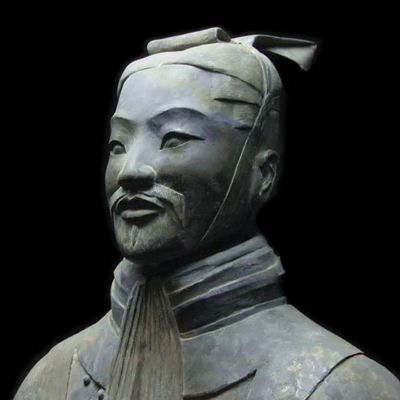
\includegraphics[width=1.9cm]{../ressources/sun_tzu_general}
  };
\end{tikzpicture}
\begin{quote}“L'art de la guerre, c'est de soumettre l'ennemi sans combat.”\end{quote}
\vfill
\begin{columns}[t]
\begin{column}{0.5\linewidth}
Préceptes
\begin{itemize}
\item prendre toutes les possessions de l'adversaire et les conserver intactes
\item adaptabilité, préparation, connaissance du terrain et des forces en présence (espionnage)
\end{itemize}
\end{column}
\begin{column}{0.5\linewidth}
Axes stratégiques
\begin{enumerate}
\item cause morale
\item conditions climatiques
\item conditions géographiques
\item qualités du dirigeant
\item organisation et discipline
\end{enumerate}
\end{column}
\end{columns}

\footlineextra{\cite{tzu1997art, sun_tzu_fighting, sun_tzu_wiki}}
\end{frame}

\begin{frame}{Alexandre le grand}
\framesubtitle{Grèce (\siecle{4} BC)}
\begin{tikzpicture}[remember picture,overlay]
	\node[anchor=north east,inner sep=0pt] at ($(current page.north east)+(-0.1cm,-0.75cm)$) {
	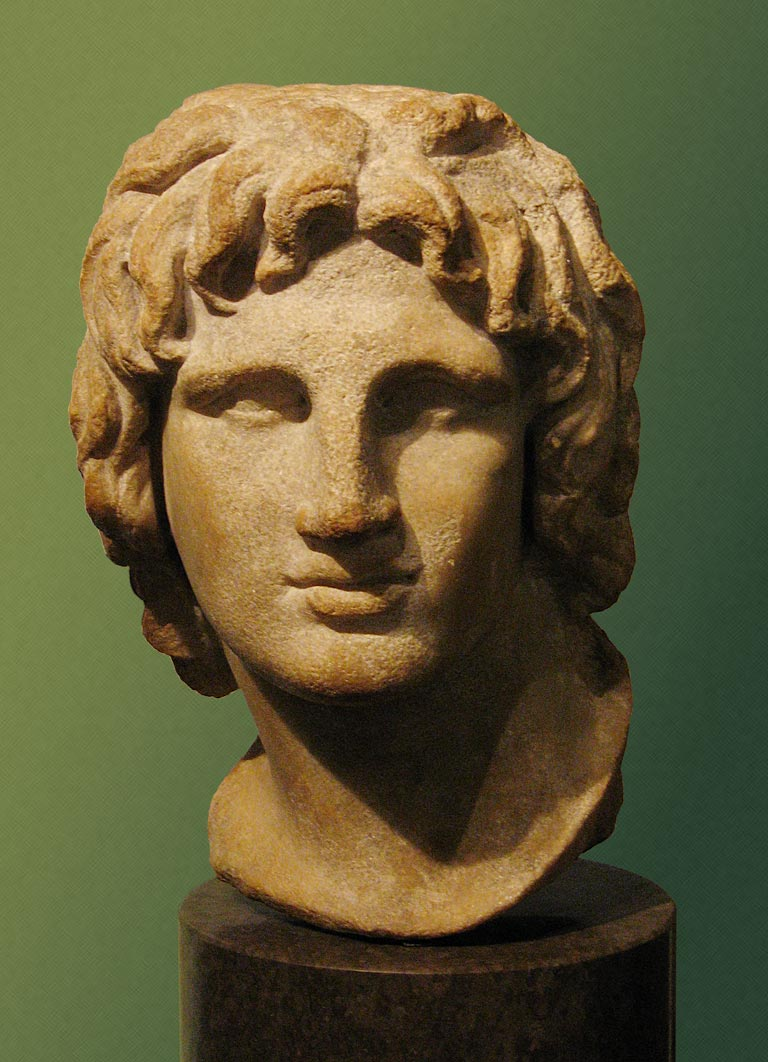
\includegraphics[trim=0cm 8cm 0cm 0cm, clip=true, width=1.9cm]{../ressources/AlexanderTheGreat_Bust}
  };
\end{tikzpicture}
\begin{quote}“Ce qui ne me tue pas me rend plus fort.”\end{quote}
\vfill
\begin{columns}[t]
\begin{column}{0.5\linewidth}
Préceptes
\begin{itemize}
\item conscription et intégration des peuples vaincus
\item allègement de l'équipement des troupes
\end{itemize}
\end{column}
\begin{column}{0.5\linewidth}
Axes stratégiques
\begin{enumerate}
\item assurer ses arrières
\item choisir judicieusement la voie d'accès pour chaque conquête
\end{enumerate}
\end{column}
\end{columns}
\footlineextra{\cite{alexander_the_great, alexandre_balkans}}
\end{frame}

\begin{frame}{Julius Caesar}
\framesubtitle{Italie (\siecle{1} BC)}
\begin{tikzpicture}[remember picture,overlay]
	\node[anchor=north east,inner sep=0pt] at ($(current page.north east)+(-0.1cm,-0.75cm)$) {
	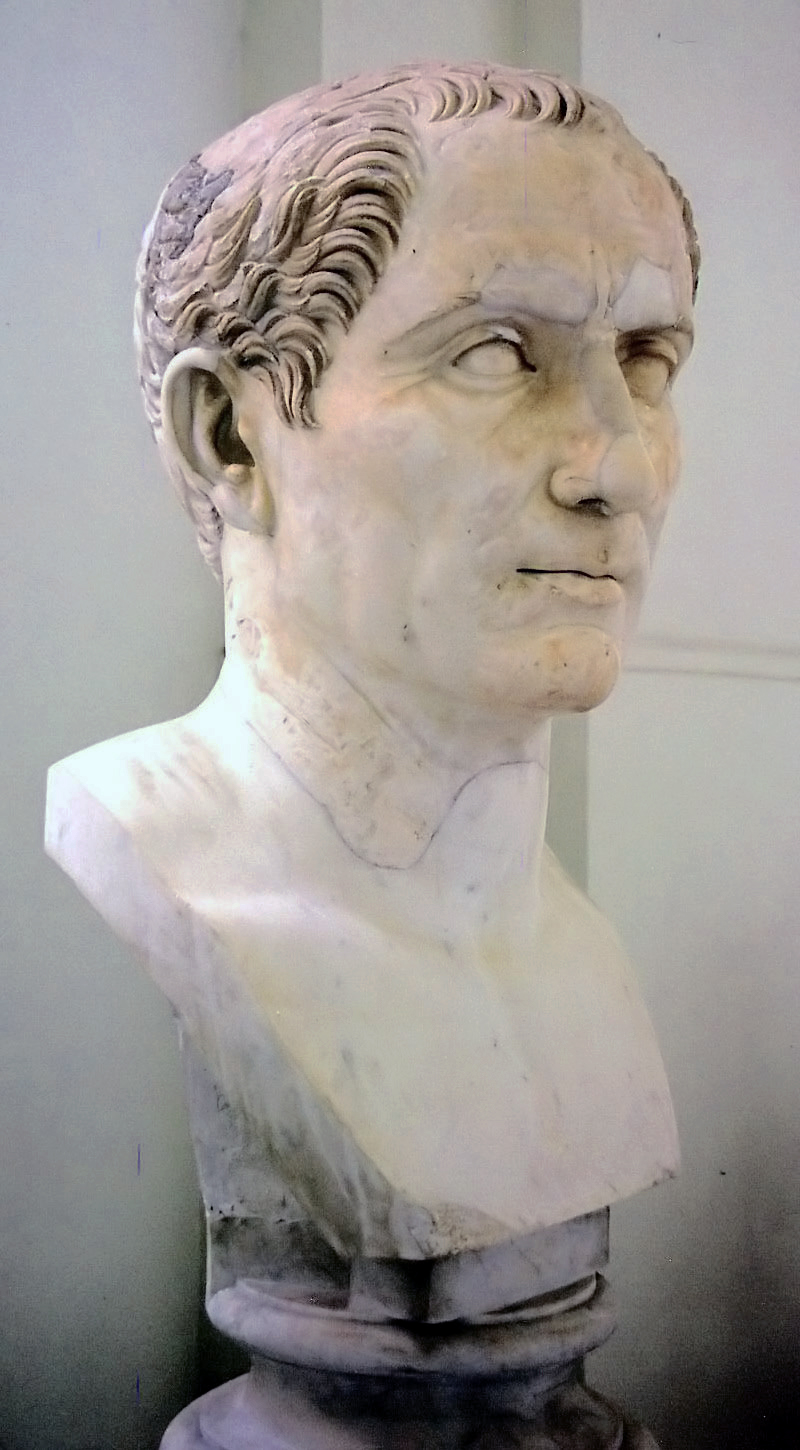
\includegraphics[trim=0cm 20cm 0cm 0cm, clip=true, width=1.9cm]{../ressources/cesare}
  };
\end{tikzpicture}
\begin{quote}“L’expérience, voilà le maître en toutes choses.”\end{quote}
\vfill
\begin{columns}[t]
\begin{column}{0.5\linewidth}
Préceptes
\begin{itemize}
\item stabilité militaire et logistique
\end{itemize}
\end{column}
\begin{column}{0.5\linewidth}
Axes stratégiques
\begin{enumerate}
\item infanterie lourde
\item bataillons étrangers spécialisés
\item formations en fonction des conditions géographiques
\item bivouac fortifié
\end{enumerate}
\end{column}
\end{columns}
\footlineextra{\cite{caesar_wiki, caesar_lacks}}
\end{frame}

\begin{frame}{Genghis Khan}
\framesubtitle{Mongolie (\siecle{12})}
\begin{tikzpicture}[remember picture,overlay]
	\node[anchor=north east,inner sep=0pt] at ($(current page.north east)+(-0.1cm,-0.75cm)$) {
	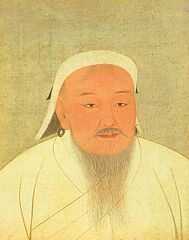
\includegraphics[trim=0cm 1cm 0cm 1cm, clip=true, width=1.9cm]{../ressources/genghis_khan}
  };
\end{tikzpicture}
\begin{quote}“Le plus grand bonheur du Mongol est de vaincre l’ennemi, de ravir ses trésors, de faire hurler ses serviteurs, de se sauver au galop de ses chevaux bien nourris [\ldots]”\end{quote}
\vfill
\begin{columns}[t]
\begin{column}{0.5\linewidth}
Préceptes
\begin{itemize}
\item guerre psychologique
\item règne de la terreur
\item connaissance du terrain : espionnage ; éclaireurs
\end{itemize}
\end{column}
\begin{column}{0.5\linewidth}
Axes stratégiques
\begin{enumerate}
\item peu de troupes ; avant-garde forte
\item troupes montées % logistique et vitesse
\item délégation des décisions
\item relais de communication et ravitaillement
\item attaques biologiques
\end{enumerate}
\end{column}
\end{columns}
\footlineextra{\cite{khan_wiki, military_strategy, mongol_army}}
\end{frame}

\begin{frame}{Napoléon Bonaparte}
\framesubtitle{France (\siecle{18})}
\begin{tikzpicture}[remember picture,overlay]
	\node[anchor=north east,inner sep=0pt] at ($(current page.north east)+(-0.1cm,-0.75cm)$) {
	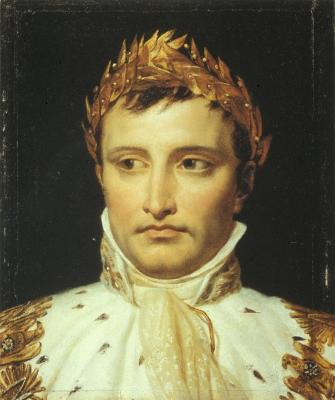
\includegraphics[trim=0cm 2cm 0cm 0cm, clip=true, width=1.9cm]{../ressources/napoleon}
  };
\end{tikzpicture}
\begin{quote}“Réunir ses feux contre un seul point ; une fois la brèche faite, l’équilibre est rompu, tout le reste devient inutile.”\end{quote}
\vfill
\begin{columns}[t]
\begin{column}{0.5\linewidth}
Préceptes
\begin{itemize}
\item recherche systématique de la bataille
\item destruction totale des forces adverses
\item être le plus fort à l’endroit où l’on a décidé de frapper le coup décisif
\end{itemize}
\end{column}
\begin{column}{0.5\linewidth}
Axes stratégiques
\begin{enumerate}
\item vitesse de manœuvre : {\emph Blitzkrieg}
\item fortifications
\item lignes de réapprovisionnement provisoires
\item artillerie
\end{enumerate}
\end{column}
\end{columns}
\footlineextra{\cite{napoleon, napoleon_wiki, napoleon_portrait}}
\end{frame}

\begin{frame}{Synthèse}
\emph{Consensus sur les points stratégiques suivants :}
\begin{itemize}
\item connaissance du terrain et des forces en présence
\item organisation et discipline
\item choix politique et géographique de la voie de progression
\end{itemize}
\vfill
\emph{Choix stratégiques opposés :}

\bigskip
\begin{tabular}{rl}
adaptabilité, délégation, flexibilité & organisation rigide\\
absorption et intégration de l'adversaire & le détruire et le terroriser\\
troupes légères et mobiles & troupes lourdes\\
campements provisoires & fortifications\\
effectifs réduits & armée expansive\\
\end{tabular}
\end{frame}


\subsection{Tactiques}
\begin{frame}{test}

\end{frame}


\section{Applications aux systèmes multi-agents}


\section{Bibliographie}
\bibliographystyle{plain}
%\bibliographystyle{amsalpha}
\begin{frame}[allowframebreaks]
\frametitle{Bibliographie}
\bibliography{../Bib.bib}
\end{frame}

\end{document}


